\subsection{Analyzing entropy in Mathematica}
\newcommand{\EntropyGfxScale}{0.8\textwidth}

(This part has been first appeared in my blog at 13-May-2015.
Some discussion: \url{https://news.ycombinator.com/item?id=9545276}.)

It is possible to slice a file by blocks, calculate entropy of each and draw a graph.
I did this in Wolfram Mathematica for demonstration and here is a source code (Mathematica 10):

\begin{lstlisting}[style=custommath]
(* loading the file *)
input=BinaryReadList["file.bin"];

(* setting block sizes *)
BlockSize=4096;BlockSizeToShow=256;

(* slice blocks by 4k *)
blocks=Partition[input,BlockSize];

(* how many blocks we've got? *)
Length[blocks]

(* calculate entropy for each block. 2 in Entropy[] (base) is set with the intention so Entropy[] 
function will produce the same results as Linux ent utility does *)
entropies=Map[N[Entropy[2,#]]&,blocks];

(* helper functions *)
fBlockToShow[input_,offset_]:=Take[input,{1+offset,1+offset+BlockSizeToShow}]
fToASCII[val_]:=FromCharacterCode[val,"PrintableASCII"]
fToHex[val_]:=IntegerString[val,16]
fPutASCIIWindow[data_]:=Framed[Grid[Partition[Map[fToASCII,data],16]]]
fPutHexWindow[data_]:=Framed[Grid[Partition[Map[fToHex,data],16],Alignment->Right]]

(* that will be the main knob here *)
{Slider[Dynamic[offset],{0,Length[input]-BlockSize,BlockSize}],Dynamic[BaseForm[offset,16]]}

(* main UI part *)
Dynamic[{ListLinePlot[entropies,GridLines->{{-1,offset/BlockSize,1}},Filling->Axis,AxesLabel->{"offset","entropy"}],
CurrentBlock=fBlockToShow[input,offset];
fPutHexWindow[CurrentBlock],
fPutASCIIWindow[CurrentBlock]}]
\end{lstlisting}

\subsubsection{GeoIP ISP database}

\myindex{GeoIP}
Let's start with the \href{https://www.maxmind.com/en/geoip-demo}{GeoIP} file (which assigns ISP to the block of IP addresses).
This binary file \IT{GeoIPISP.dat} has some tables (which are IP address ranges perhaps)
plus some text blob at the end of the file (containing ISP names).

When I load it to Mathematica, I see this:

\begin{figure}[H]
\centering
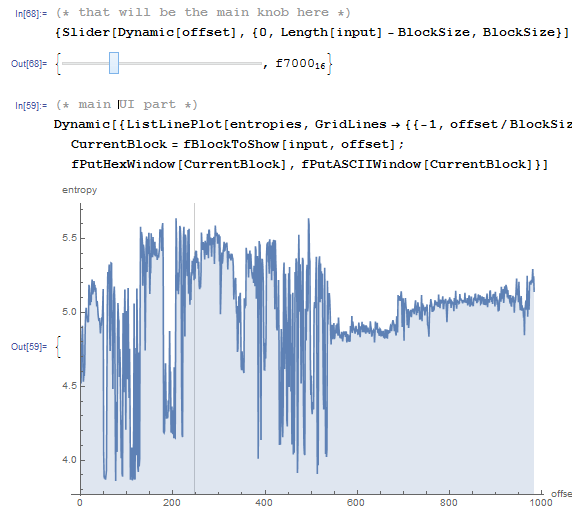
\includegraphics[width=\EntropyGfxScale]{ff/entropy/geoipisp11.png}
\end{figure}

\begin{figure}[H]
\centering
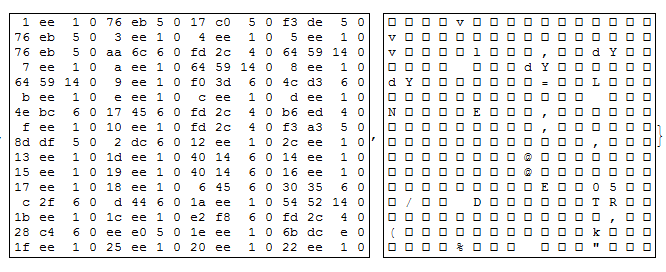
\includegraphics[width=\EntropyGfxScale]{ff/entropy/geoipisp12.png}
\end{figure}


There are two parts in graph: first is somewhat chaotic, second is more steady.

0 in horizontal axis in graph means lowest entropy
(the data which can be compressed very tightly, \IT{ordered} in other words) 
and 8 is highest (cannot be compressed at all, \IT{chaotic} or \IT{random} in other words).
Why 0 and 8? 0 means 0 bits per byte (byte as a container is not filled at all) 
and 8 means 8 bits per byte, i.e., the whole byte container is filled with the information tightly.

So I put slider to point in the middle of the first block, and I clearly see some array of 32-bit integers.
Now I put slider in the middle of the second block and I see English text:

\begin{figure}[H]
\centering
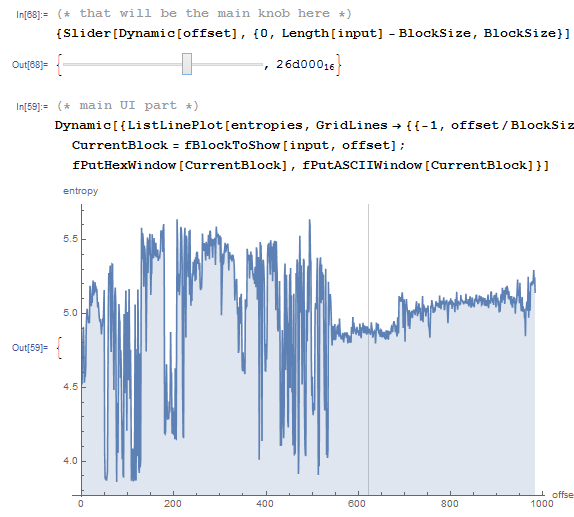
\includegraphics[width=\EntropyGfxScale]{ff/entropy/geoipisp21.png}
\end{figure}

\begin{figure}[H]
\centering
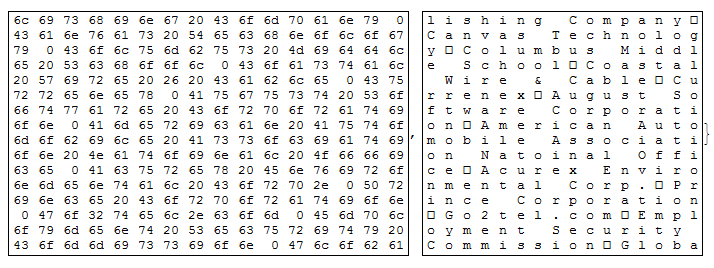
\includegraphics[width=\EntropyGfxScale]{ff/entropy/geoipisp22.png}
\end{figure}


Indeed, this are names of ISPs.
So, entropy of English text is 4.5-5.5 bits per byte? Yes, something like this.
Wolfram Mathematica has some well-known English literature corpus embedded, and we can see entropy of Shakespeare's sonnets:

\begin{lstlisting}[style=custommath]
In[]:= Entropy[2,ExampleData[{"Text","ShakespearesSonnets"}]]//N
Out[]= 4.42366
\end{lstlisting}

4.4 is close to what we've got (4.7-5.3). 
Of course, classic English literature texts are somewhat different from ISP names and other
English texts we can find in binary files 
(debugging/logging/error messages), but this value is close.

\subsubsection{TP-Link WR941 firmware}

Next example. I've got firmware for TP-Link WR941 router:

\begin{figure}[H]
\centering
\includegraphics[width=\EntropyGfxScale]{ff/entropy/tplink.png}
\end{figure}


We see here 3 blocks with empty lacunas.
Then the first block with high entropy (started at address 0) is small, second (address somewhere at 0x22000) is bigger and third (address 0x123000) is biggest.
I can't be sure about exact entropy of the first block, but 2nd and 3rd has very high entropy, meaning that these blocks are either
compressed and/or encrypted.

\myindex{Binwalk}
I tried \href{http://binwalk.org/}{binwalk} for this firmware file:

\begin{lstlisting}
DECIMAL       HEXADECIMAL     DESCRIPTION
--------------------------------------------------------------------------------
0             0x0             TP-Link firmware header, firmware version: 0.-15221.3, image version: "", product ID: 0x0, product version: 155254789, kernel load address: 0x0, kernel entry point: 0x-7FFFE000, kernel offset: 4063744, kernel length: 512, rootfs offset: 837431, rootfs length: 1048576, bootloader offset: 2883584, bootloader length: 0
14832         0x39F0          U-Boot version string, "U-Boot 1.1.4 (Jun 27 2014 - 14:56:49)"
14880         0x3A20          CRC32 polynomial table, big endian
16176         0x3F30          uImage header, header size: 64 bytes, header CRC: 0x3AC66E95, created: 2014-06-27 06:56:50, image size: 34587 bytes, Data Address: 0x80010000, Entry Point: 0x80010000, data CRC: 0xDF2DBA0B, OS: Linux, CPU: MIPS, image type: Firmware Image, compression type: lzma, image name: "u-boot image"
16240         0x3F70          LZMA compressed data, properties: 0x5D, dictionary size: 33554432 bytes, uncompressed size: 90000 bytes
131584        0x20200         TP-Link firmware header, firmware version: 0.0.3, image version: "", product ID: 0x0, product version: 155254789, kernel load address: 0x0, kernel entry point: 0x-7FFFE000, kernel offset: 3932160, kernel length: 512, rootfs offset: 837431, rootfs length: 1048576, bootloader offset: 2883584, bootloader length: 0
132096        0x20400         LZMA compressed data, properties: 0x5D, dictionary size: 33554432 bytes, uncompressed size: 2388212 bytes
1180160       0x120200        Squashfs filesystem, little endian, version 4.0, compression:lzma, size: 2548511 bytes, 536 inodes, blocksize: 131072 bytes, created: 2014-06-27 07:06:52
\end{lstlisting}

\myindex{LZMA}
Indeed: there are some stuff at the beginning, but two large LZMA compressed blocks are started at 0x20400 and 0x120200.
These are roughly addresses we have seen in Mathematica.
Oh, and by the way, binwalk can show entropy information as well (\TT{-E} option):

\begin{lstlisting}
DECIMAL       HEXADECIMAL     ENTROPY
--------------------------------------------------------------------------------
0             0x0             Falling entropy edge (0.419187)
16384         0x4000          Rising entropy edge (0.988639)
51200         0xC800          Falling entropy edge (0.000000)
133120        0x20800         Rising entropy edge (0.987596)
968704        0xEC800         Falling entropy edge (0.508720)
1181696       0x120800        Rising entropy edge (0.989615)
3727360       0x38E000        Falling entropy edge (0.732390)
\end{lstlisting}

Rising edges are corresponding to rising edges of block on our graph.
Falling edges are the points where empty lacunas are started.

Binwalk can also generate PNG graphs (\TT{-E -J}):

\begin{figure}[H]
\centering
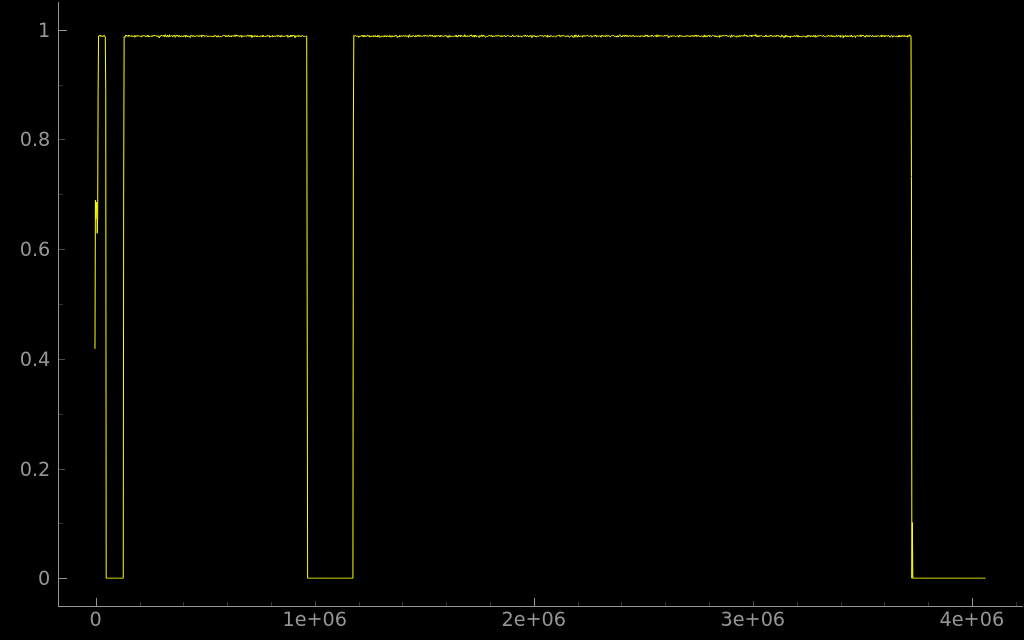
\includegraphics[width=\EntropyGfxScale]{ff/entropy/tplink_binwalk.png}
\end{figure}


What can we say about lacunas? By looking in hex editor, we see that these are just filled with 0xFF bytes.
Why developers put them?
Perhaps, because they weren't able to calculate precise compressed blocks sizes, so they allocated space
for them with some reserve.

\subsubsection{Notepad}

\myindex{Notepad}

Another example is notepad.exe I've picked in Windows 8.1:

\begin{figure}[H]
\centering
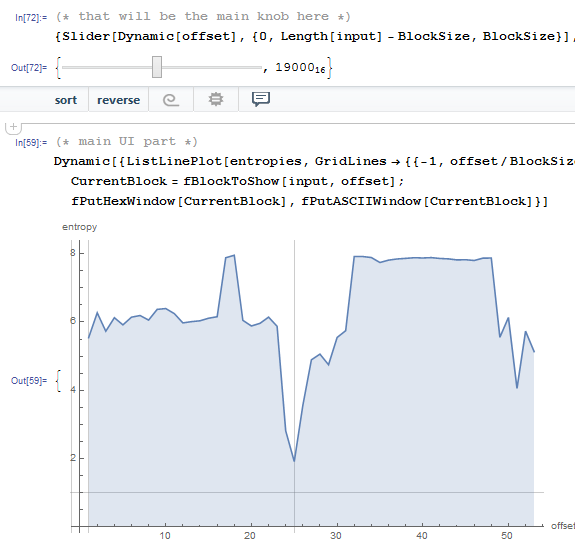
\includegraphics[width=\EntropyGfxScale]{ff/entropy/notepad11.png}
\end{figure}

\begin{figure}[H]
\centering
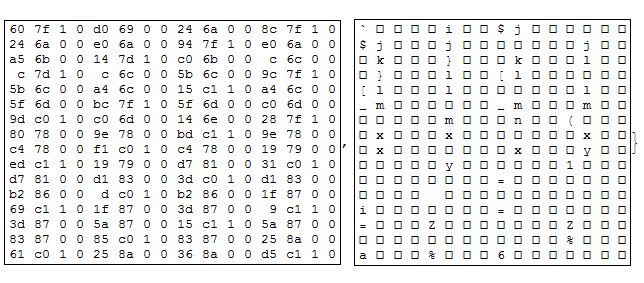
\includegraphics[width=\EntropyGfxScale]{ff/entropy/notepad12.png}
\end{figure}


There is cavity at $\approx 0x19000$ (absolute file offset).
I've opened the executable file in hex editor and found imports table there (which has lower entropy than x86-64 code
in the first half of graph).

There are also high entropy block started at $\approx 0x20000$:

\begin{figure}[H]
\centering
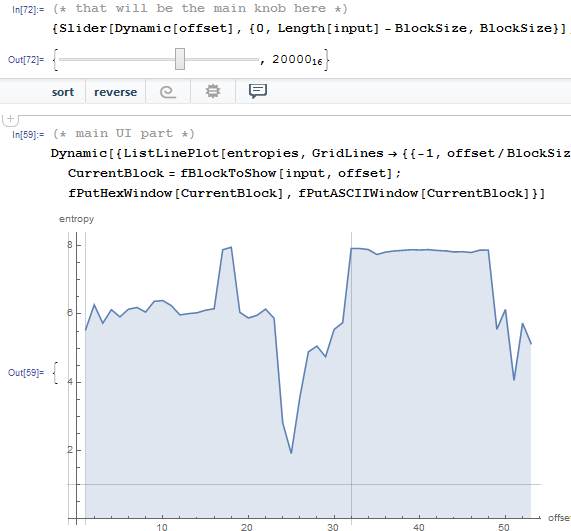
\includegraphics[width=\EntropyGfxScale]{ff/entropy/notepad21.png}
\end{figure}

\begin{figure}[H]
\centering
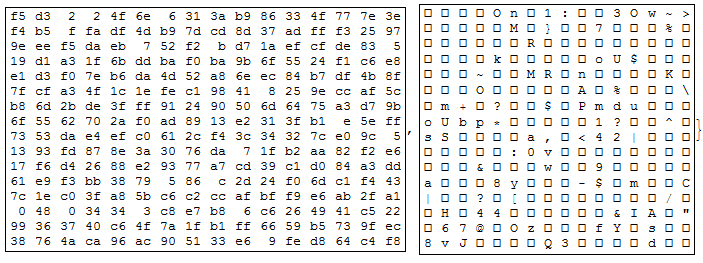
\includegraphics[width=\EntropyGfxScale]{ff/entropy/notepad22.png}
\end{figure}


\myindex{PNG}
In hex editor I can see PNG file here, embedded in the PE file resource section (it is a large image of notepad icon).
PNG files are compressed, indeed.

\subsubsection{Unnamed dashcam}

Now the most advanced example in this part is the firmware of some unnamed dashcam I've received from friend:

\begin{figure}[H]
\centering
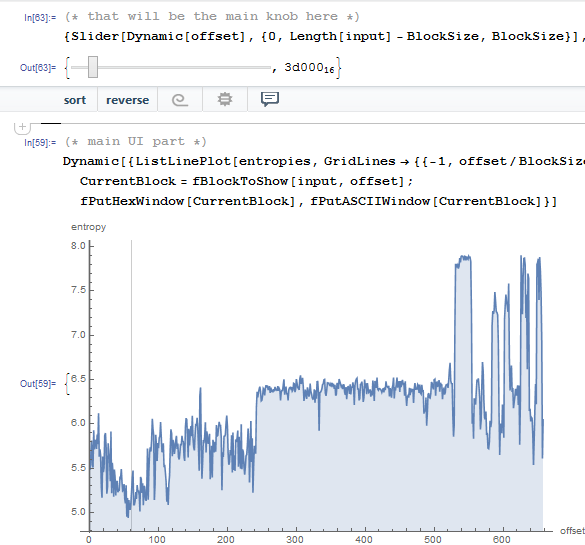
\includegraphics[width=\EntropyGfxScale]{ff/entropy/dashcam_text1.png}
\end{figure}

\begin{figure}[H]
\centering
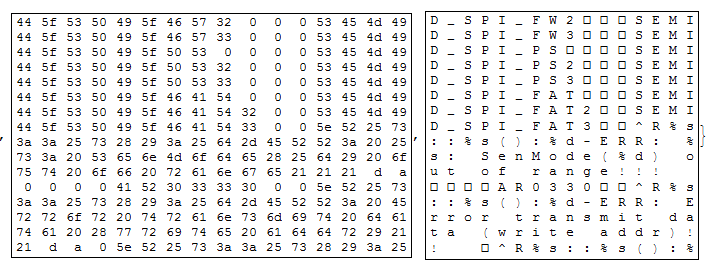
\includegraphics[width=\EntropyGfxScale]{ff/entropy/dashcam_text2.png}
\end{figure}


The cavity at the very beginning is an English text: debugging messages.
\myindex{MIPS}
I checked various \ac{ISA}s and I found that 
the first third of the whole file (with the text segment inside) is in fact MIPS (little-endian) code.

For instance, this is very distinctive MIPS function epilogue:

\begin{lstlisting}[style=customasmMIPS]
ROM:000013B0                 move    $sp, $fp
ROM:000013B4                 lw      $ra, 0x1C($sp)
ROM:000013B8                 lw      $fp, 0x18($sp)
ROM:000013BC                 lw      $s1, 0x14($sp)
ROM:000013C0                 lw      $s0, 0x10($sp)
ROM:000013C4                 jr      $ra
ROM:000013C8                 addiu   $sp, 0x20
\end{lstlisting}

From our graph we can see that MIPS code has entropy of 5-6 bits per byte.
Indeed, I once measured various \ac{ISA}s entropy and I've got these values:

\begin{itemize}
\item x86: .text section of ntoskrnl.exe file from Windows 2003: 6.6
\item x64: .text section of ntoskrnl.exe file from Windows 7 x64: 6.5
\item ARM (thumb mode), Angry Birds Classic: 7.05
\item ARM (ARM mode) Linux Kernel 3.8.0: 6.03
\item MIPS (little endian), .text section of user32.dll from Windows NT 4: 6.09
\end{itemize}

So the entropy of executable code is higher than of English text, but still can be compressed.

Now the second third is started at 0xF5000. I don't know what this is. I tried different \ac{ISA}s but without success.
The entropy of the block is looks even steadier than for executable one.
Maybe some kind of data?

\myindex{JPEG}
There is also a spike at $\approx 0x213000$.
I checked it in hex editor and I found JPEG file there (which, of course, compressed)!
I also don't know what is at the end.
Let's try Binwalk for this file:

\begin{lstlisting}
% binwalk FW96650A.bin 

DECIMAL       HEXADECIMAL     DESCRIPTION
--------------------------------------------------------------------------------
167698        0x28F12         Unix path: /15/20/24/25/30/60/120/240fps can be served..
280286        0x446DE         Copyright string: "Copyright (c) 2012 Novatek Microelectronic Corp."
2169199       0x21196F        JPEG image data, JFIF standard 1.01
2300847       0x231BAF        MySQL MISAM compressed data file Version 3

% binwalk -E FW96650A.bin 

DECIMAL       HEXADECIMAL     ENTROPY
--------------------------------------------------------------------------------
0             0x0             Falling entropy edge (0.579792)
2170880       0x212000        Rising entropy edge (0.967373)
2267136       0x229800        Falling entropy edge (0.802974)
2426880       0x250800        Falling entropy edge (0.846639)
2490368       0x260000        Falling entropy edge (0.849804)
2560000       0x271000        Rising entropy edge (0.974340)
2574336       0x274800        Rising entropy edge (0.970958)
2588672       0x278000        Falling entropy edge (0.763507)
2592768       0x279000        Rising entropy edge (0.951883)
2596864       0x27A000        Falling entropy edge (0.712814)
2600960       0x27B000        Rising entropy edge (0.968167)
2607104       0x27C800        Rising entropy edge (0.958582)
2609152       0x27D000        Falling entropy edge (0.760989)
2654208       0x288000        Rising entropy edge (0.954127)
2670592       0x28C000        Rising entropy edge (0.967883)
2676736       0x28D800        Rising entropy edge (0.975779)
2684928       0x28F800        Falling entropy edge (0.744369)
\end{lstlisting}

Yes, it found JPEG file and even MySQL data!
But I'm not sure if it's true---I didn't check it yet.

\myindex{clusterization}
It's also interesting to try clusterization in Mathematica:

\begin{figure}[H]
\centering
\includegraphics[width=\EntropyGfxScale]{ff/entropy/dashcam_clusters.png}
\end{figure}


Here is an example of how Mathematica grouped various entropy values into distinctive groups.
Indeed, there is something credible. Blue dots in range of 5.0-5.5 are supposedly related to English text.
Yellow dots in 5.5-6 are MIPS code. A lot of green dots in 6.0-6.5 is the unknown second third.
Orange dots close to 8.0 are related to compressed JPEG file.
Other orange dots are supposedly related to the end of the firmware (unknown to us data).

\subsubsection{Links}

Binary files used in this part: \url{https://github.com/DennisYurichev/RE-for-beginners/tree/master/ff/entropy/files}.
Wolfram Mathematica notebook file: \url{https://github.com/DennisYurichev/RE-for-beginners/blob/master/ff/entropy/files/binary_file_entropy.nb}
(all cells must be evaluated to start things working).

